\problemname{Dark Ride}

Erika recently got a summer job at the amusement park Phantasialand near Bonn.
She was hired to control the lights in the rooms through which a dark ride passes.

The ride passes through $N$ rooms, numbered from $0$ to $N-1$. The rooms are traversed in order, starting in room $0$ and ending in room $N-1$. The lights in the rooms are controlled by $N$ switches (also numbered from $0$ to $N-1$), one for each room. Switch $s$ (where $0\le s < N$) controls the light in room $p_{s}$.

Erika's boss has asked her to turn on the lights in the first and last rooms and turn off all the others. Sounds easy, right? She just needs to turn on the two switches $A$ and $B$ such that $p_{A} = 0$ and $p_{B} = N-1$ (or $p_{B} = 0$ and $p_{A} = N-1$). Unfortunately, Erika did not fully pay attention when her boss described the controls, and \textbf{she does not remember the array $p$ -- that is, which switch controls which room}.

Erika needs to figure this out before her boss notices.
Before the start of each ride, Erika turns off all the lights and can then turn on a subset of the switches. As the ride goes from room to room, whenever the ride goes from a lit room to an unlit room or vice versa, Erika will hear the passengers scream in excitement. The speed of the ride can vary, so Erika cannot directly infer which rooms are lit but at least she will hear the number of screams. That is, she will learn the number of times the ride passes from lit to unlit room, or unlit to lit room.

Can you help Erika figure out which two switches control the lights for the first and last rooms before her boss notices?  You can use at most $30$ rides.

\section*{Interaction}
This is an interactive problem.

\begin{itemize}

  \item
Your program should start by reading a line with an integer $N$: the number of rooms in the dark ride.

  \item
Then, your program should interact with the grader.
    To start a ride, you should print a line beginning with a question mark `\verb!?!', and then a string of length $N$ consisting of \verb!0!'s (turned off) and \verb!1!’s (turned on) indicating how you set the $N$ switches.
Then, your program should read a single integer $\ell$ ($0 \leq \ell < N$), the number of times Erika hears the passengers scream.

  \item
    When you want to answer, print a line with an exclamation mark `\verb|!|', followed by two integers $A$ and $B$ ($0\le A,B < N$). For your answer to be accepted, these must be the indices of the switches controlling the two end rooms, in any order.
After this, your program should exit.
\end{itemize}

The grader is non-adaptive, meaning that the hidden array $p$ is determined before the interaction begins.

Make sure to flush standard output after issuing each ride, or else your program might get judged as Time Limit Exceeded.
In Python, this happens automatically as long as you use \verb@input()@ to read lines. In C++, \verb@cout << endl;@ flushes in addition to printing a newline; if using printf, use \texttt{fflush(stdout)}.


\section*{Constraints and Scoring}
\begin{itemize}
  \item  $3 \le N \le 30\,000$.
  \item You can issue at most $30$ rides (printing the final answer does not count as a ride). If you exceed this, you will get the verdict `Wrong Answer'.
\end{itemize}

\noindent
Your solution will be tested on a set of test groups, each worth a number of points.
Each test group contains a set of test cases. To get the points for a test group, you need to solve all test cases in the test group.

\noindent
\begin{tabular}{| l | l | l |}
\hline
Group & Score & Limits \\ \hline
  1 & 9 & $N = 3$ \\ \hline
  2 & 15 & $N \le 30$ \\ \hline
  3 & 17 & $p_{0} = 0$, i.e., switch $0$ controls room $0$ \\ \hline
  4 & 16 & $N$ is even, with one output switch in the first half ($0 \le A < \frac{N}{2}$) and one in the second half ($\frac{N}{2} \le B < N$)  \\ \hline
  5 & 14 & $N \le 1000$ \\ \hline
  6 & 29 & No additional constraints  \\ \hline
\end{tabular}


\section*{Testing Tool}
To facilitate the testing of your solution, we have provided a simple tool that you can download.
See `attachments' at the bottom of the Kattis problem page. The tool is optional to use. Note that the official Kattis grader differs from the provided testing tool.

To use the tool, create an input file, such as `sample1.in', which should start with a number $N$ followed by a line with $p_{0}, p_{1}, \ldots, p_{N-1}$ specifying the hidden permutation. For example:

\begin{verbatim}
    5
    2 1 0 3 4
 \end{verbatim}
 
 
 \noindent
 For Python programs, say \verb|solution.py| (normally run as \verb|pypy3 solution.py|):
 
     \verb|python3 testing_tool.py pypy3 solution.py < sample1.in|
 
 \noindent
 For C++ programs, first compile it
 (e.g.\ with \verb|g++ -g -O2 -std=gnu++23 -static solution.cpp -o solution.out|)
 and then run:
 
     \verb|python3 testing_tool.py ./solution.out < sample1.in|
 
\section*{Example}
In the first sample, the hidden permutation is $[p_{0},p_{1},p_{2},p_{3},p_{4}] = [2,1,0,3,4]$.
This satisfies the constraints of test groups 2, 5, and 6.
First, the program reads the integer $N = 5$. Then, the program requests a ride with two turned on switches: switch $4$ and switch $0$. These control rooms $p_{4} = 4$
and $p_{0} = 2$; see the illustration below. Erika hears $3$ screams (marked by arrows in the figure): first when the ride passes from unlit room $1$ to lit room $2$; second from lit room $2$ to unlit room $3$; and thirdly when passing from unlit room 3 to lit room $4$. The program then requests another ride where rooms $p_{0},p_{2}$, and $p_{3}$ are lit, making Erika hear $3$ screams. Finally, the program answers with $A = 2$ and $B = 4$, which is indeed correct as these control the first and last rooms ($p_{2} = 0$ and $p_{4} = 4$). Note that $A = 4$ and $B = 2$ would also have been a correct answer.

  
\begin{center}
    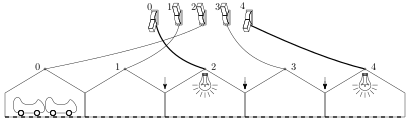
\includegraphics[width=0.9\textwidth]{sample.pdf}
  \end{center}

In the second sample, the hidden permutation is $[p_{0},p_{1},p_{2}] = [2,0,1]$.
This satisfies the constraints of test groups 1, 2, 5, and 6.
The program requests a ride where all three switches are turned on. Since this means all the rooms are lit, Erika will hear no screams. In the second ride, switches $1$ and $0$ are turned on, making rooms $p_{1} = 0$ and $p_{0} = 2$ be lit, while room $1$ is unlit. Erika hears two screams: when the ride goes from room $0$ (lit) to room $1$ (unlit), and from room $1$ (unlit) to room $2$ (lit). In the final ride, no switches are turned on, meaning that all three rooms are unlit, and again that Erika hears no screams. The program then answers with switches $1$ and $0$, which indeed control the first and last room. Both `\verb|! 0 1|' and `\verb|! 1 0|' are accepted answers.

In the third sample, the hidden permutation is $[p_{0},p_{1},p_{2},p_{3}] = [0,1,2,3]$. This satisfies the constraints of test groups 2, 3, 4, 5, and 6. Note that it is not necessarily possible to infer the answer after this one ride, but the sample solution guessed the answer and got lucky.
